%!TEX program = xelatex
%!TEX root = ../thesis.tex
\chapter{Related Work}\label{chap:related_work}

As air pollution problems arise in recent years, people pay more and more attention to air quality issues. Many research and engineering work has been carried out. As for a most instinctive view, Figure \ref{fig:aqi_map}  shows a web platform that visualizes the real-time air quality data on the world map.
% \yan{I think it should be Figure~\ref{fig:aqi_map}, Figure X, not FigureX.}

\begin{figure}[!htbp]
    \centering
    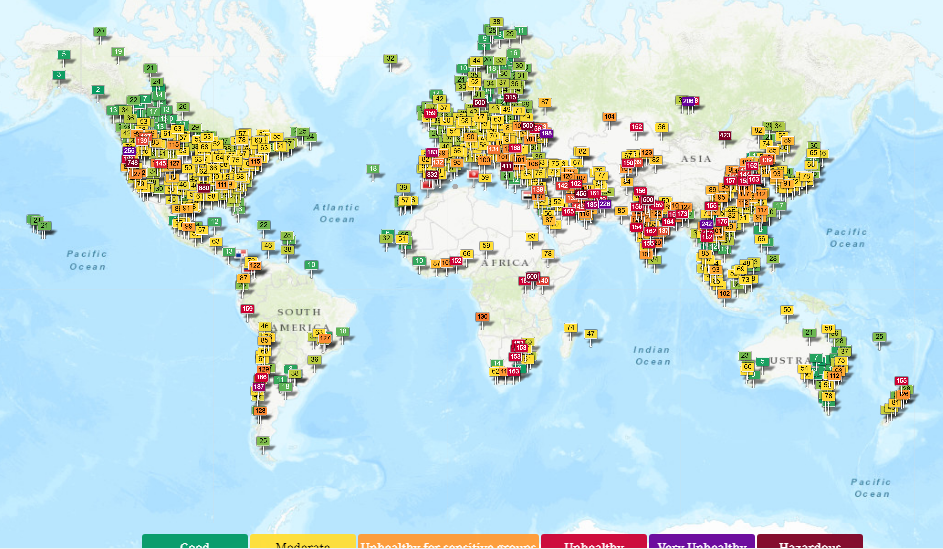
\includegraphics[width=0.7\linewidth]{fig/air-pollution-map-Screenshot-2021-08-11-020331.png}
    \caption{Real-time Air Quality Index Visual Map \cite{aqi_map}. From left to right, green, yellow, orange, red, purple, and brown represent AQI levels of good, moderate, unhealthy for sensitive groups, unhealthy, very unhealthy, and hazardous, respectively. Website: \href{https://aqicn.org/map/world/}{https://aqicn.org/map/world/}}
    \label{fig:aqi_map}
\end{figure}

We can have a clear view of the real-time air quality status from the website, city by city. However, how these data are collected, synthesized, and what's their use are all questions. In general, current engineering and academic works could be divided into several areas:

\begin{itemize}
% \yan{maybe need to define MIMO before using this abbreviation}
    \item \textbf{IoT system design for data collecting}. An IoT system is a must as an ending unit for data collecting, integrated by a bottom layer processing unit such as MIMO, ARM, or Arduino. Of course, a sensor capable of measuring and retrieving real-time (e.g., 1 Hz) air pollution data is the basic. Peripheral work such as sensor device and circuits design is also very important for data reliability.
    \item \textbf{Sensor network design, planning and optimization}. From a global view, we can check the air pollution status from a city to another. However, sometimes, we have different scenario-related demands. For example, when we want to more precisely analyze the city's pollution status, maybe thousands of sensors should be arranged in a large area. The problem here is sensor network designing.
    \item \textbf{Time series forecasting}. This is the topic that this thesis concerns. When we have collected enough real and reliable air pollution data, the first idea is to do data fitting and predict their trends. Only with these predictions can we make public decisions, pay attention to the causes of these air pollution problems, and rethink how to prevent them.
\end{itemize}

In this chapter, we'll give a brief introduction to these works.
% \yan{following with their limitations}

\section{IoT and Sensor Network for Data Collecting}
% \yan{How about $CO$, $NO_2$, $SO_2$, and $O_3$}
% \yan{I think we should have a space between AuthorName and citation. But I am not sure. You can check existing thesis.}
Kularatna et al. \cite{kularatna2008environmental} built an environmental air pollution monitoring system for monitoring the concentrations of major air pollutants, which complies with the IEEE 1451.2 standard. This system can measure concentrations of gases such as $CO$, $NO_2$, $SO_2$, and $O_3$ using semiconductor sensors. Ailing et al. \cite{ailing2017design} PM2.5 detector based on ARM. The system has a PM2.5 sensor unit and has peripheral modules such as an LCD data display unit and an LED warning unit for hardware-level notification. Okokpujie et al. \cite{okokpujie2018smart} also developed a smart air pollution monitoring system using Arduino.

Regarding the placing problems of sensors, Kanaroglou \cite{KANAROGLOU20052399} et al. brought out a method of optimally locating a dense network of air pollution monitoring stations. They considered related land use, population, and biophysical information on planning the sensor network. For indoor scenarios, Bhattacharya \cite{bhattacharya2012indoor} et al. developed a wireless solution for indoor air quality monitoring in a smart building. They also developed a toolkit to view the live air quality data of deployed regions. Ray et al. \cite{ray2016internet} also built a smart PM2.5 density monitoring system based on cloud platforms.
% \cite{khedo2010wireless} et al. designed a wireless sensor network to 

When putting these research works into real applications such as civic living, Xu, Susu, et al. \cite{xu2019ilocus} creatively made advantage of ubiquitous taxi cars in cities. They combined cluster scheduling and sensor network technologies to track pollution information in the cities. They also built a cloud platform to manage the retrieved data.
% \yan{Can we add some sentences to summary the limitations of above-mentioned works? For instance: Although above-mentioned works address the problems of xxx, however, they either require xx or cannot handle xx. Thus, a novel air xx (our work) should be proposed.}
% TODO later

\section{Time Series Fitting and Forecasting}

In the last section, we survey many works regarding data gathering, which is related to fields such as IoT development, sensor network design, and big data management. These works give us baselines that show how air pollution data could be collected. In this section, we will discuss how these data could be used, especially for air pollution forecasting, based on time series fitting and forecasting.

Except for ARIMA, ETS models mentioned in our last chapter, traditional methods such as Kalman filter \cite{gomez1994estimation} are also very simple and practical for time series and forecasting problems. Random forests \cite{rouet2017machine}, XGBoost, and SVM \cite{sapankevych2009time} etc are useful machine learning methods too. About method choosing, the most suitable method is highly interrelated with the data's properties and the application scenario. 

In common, the essential of both traditional approaches and ML-based approaches is mining data and extracting features. Different from other feature engineering tasks, sliding windows are widely used for processing the data. Metrics such as the minimum, the maximum, the mean, and the variance of the data in the window are common features.
% \yan{Shall we emphasize the limitations of these methods?}

\section{Models based on Neural Networks}

The above section gave introductions to methods that cover traditional models and signal processing methods. Neural networks are proved reliable and potential since LeNet-5 \cite{lecun1998gradient} was designed for digit recognition. With the fast development of GPU hardware, more and more complex neural networks have been designed and distributed for applications. There are huge variants of neural networks applied for miscellaneous tasks such as image classification and captioning, audio recognition, video compression, video captioning, 3D point cloud processing, 3D object detection, and so on. As for time series and forecasting problems, recurrent neural networks (RNNs), Long short-term memory (LSTM) networks, deep recurrent neural network (DRNN), and convolutional neural networks (CNN) are the most common deep learning architectures that are currently being successfully applied \cite{torres2021deep}. 

LSTM-based deep learning methods have been developed recently to extract temporal patterns. Lai et al. proposed LSTNet \cite{lai2018modeling} that encodes short-term local information into low dimensional vectors using 1D convolutional neural networks and decodes the vectors through an RNN. Shih et al. proposed TPA-LSTM \cite{shih2019temporal}  which processes the inputs by an RNN and employs a convolutional neural network to calculate the attention score across multiple steps.

The architecture of CNN is designed for 2D data like images. Meanwhile, recently a special variant of CNN called temporal convolutional networks (TCNs) \cite{lea2016temporal} has been proposed that makes CNN capable for time series processing. Yan et al. \cite{yan2020temporal} released their research work about using TCN for weather forecasting in 2020 and showed that TCN is better than the LSTM network in this application.

\subsection{WaveNet Related Models}
% Put ours topic at the beginning
Recently, a series of networks related to audio applications such as speech synthesis (\cite{shen2018natural}, \cite{wang2017tacotron}) have been developed. DeepMind's WaveNet \cite{oord2016wavenet} is one of the famous and is the foundation work. They introduce a new generative model operating directly on the raw audio waveform. For WaveNet's application scenario, the joint probability of a waveform $\textbf{x}=\{x_1,x_2,...,x_T\}$ is factorized as a product of conditional probabilities as below \cite{oord2016wavenet}:

\begin{equation}
    p(\textbf{x})=\prod_{t=1}^Tp\{x_t|x_1,x_2,...,x_{t-1}\}
\end{equation}

In this model, every sample $x_t$ at any timestep is conditioned on the samples at all previous timesteps.

\subsection{Other Deep Learning Models}

WaveNet related methods, including our GreenEyes model, tackle with a single sequence of time series data and show good fitting and forecasting performance concerning the prediction accuracy and data throughput capacity. Meanwhile, same with the same recent time as this thesis was being developed, new methods and approaches regarding time series forecasting have also been proposed. In recent years, graph neural networks (GNNs) have shown high capability in handling relational dependencies. Wu et al. \cite{wu2020connecting} proposed a general graph neural network framework designed specifically for multivariate time series data. Their method is useful for extracts relations among variables belonging to multi sequences.

As Transforms \cite{vaswani2017attention} become great popular these years, another model based on Transforms has also been brought out. Lim et al. \cite{lim2021temporal} from Google introduced the Temporal Fusion Transformer (TFT) as a novel attention-based architecture which combines high-performance multi-horizon forecasting with interpretable insights into temporal dynamics. They created gate-based networks, GRN and GLU, as new approaches for better feature selection modules.
% \yan{Need to point out the relationship between these works and our proposed system. Maybe we use some of these methods. Maybe they inspire us to propose our unique method.}
